
%(BEGIN_QUESTION)
% Copyright 2010, Tony R. Kuphaldt, released under the Creative Commons Attribution License (v 1.0)
% This means you may do almost anything with this work of mine, so long as you give me proper credit

Suppose a brewery decides to install a capacitive level probe to measure the height of malt (partially germinated barley grains) in a storage silo:

$$\includegraphics[width=15.5cm]{i00318x01.eps}$$

Unfortunately, the capacitive level instrument fails to yield reliable measurements of malt height, due to variations in the malt's moisture content from delivery to delivery.  Wet malt has a greater bulk permittivity than dry malt, causing the level transmitter to register differently with the same actual height of malt inside the silo.

\vskip 10pt

The operations manager approaches you for a solution to this problem.  What do you recommend?

\vskip 20pt \vbox{\hrule \hbox{\strut \vrule{} {\bf Suggestions for Socratic discussion} \vrule} \hrule}

\begin{itemize}
\item{} When the malt is wetter but the actual malt level has not changed, will the LT register a greater level or a lesser level?  Explain why.
\item{} Are there any ways to make a capacitive instrument do a better job in this application?
\item{} For any alternative technologies you recommend, identify ways in which each one might also suffer problems when trying to measure the height of malted barley gains inside the silo.
\end{itemize}

\underbar{file i00318}
%(END_QUESTION)





%(BEGIN_ANSWER)


%(END_ANSWER)





%(BEGIN_NOTES)

Possible alternatives to a capacitance transmitter include:

\begin{itemize}
\item{} Weight (assuming variations in moisture content don't affect malt density too much)
\item{} Guided-wave radar (assuming permittivity is high enough to achieve good echo)
\item{} Float-on-retracting tape
\item{} Ultrasonic (assuming angle of repose doesn't scatter sound waves too much)
\end{itemize}

%INDEX% Measurement, level: capacitance
%INDEX% Measurement, level: radar
%INDEX% Process: brewery malt storage tank level

%(END_NOTES)


